% Copyright 2007 by Till Tantau
%
% This file may be distributed and/or modified
%
% 1. under the LaTeX Project Public License and/or
% 2. under the GNU Public License.
%
% See the file doc/licenses/LICENSE for more details.



\documentclass{beamer}

%
% DO NOT USE THIS FILE AS A TEMPLATE FOR YOUR OWN TALKS�!!
%
% Use a file in the directory solutions instead.
% They are much better suited.
%


% Setup appearance:

\usetheme{Darmstadt}
\usefonttheme[onlylarge]{structurebold}
\setbeamerfont*{frametitle}{size=\normalsize,series=\bfseries}
\setbeamertemplate{navigation symbols}{}


% Standard packages

\usepackage[english]{babel}
\usepackage[latin1]{inputenc}
\usepackage{times}
\usepackage[T1]{fontenc}


% Setup TikZ

\usepackage{tikz}
\usetikzlibrary{arrows}
\tikzstyle{block}=[draw opacity=0.7,line width=1.4cm]


% Author, Title, etc.

\title[Distributed $3$D-Print Driver] 
{%
 Distributed $\textbf{3}$D-Print Driver
 %
}

\author[Guide]{
	\textbf{Presenter}: Suman~Bidarahalli \\	
	\textbf{Supervisor}: Dr.Alan~Brunton 
}
\institute[TU Darmstadt]
{
  Technische Universit�t Darmstadt, Germany
}

\date[ Master Thesis Presentation 2016]
{Master Thesis Presentation, August 2016}



% The main document

\begin{document}

\begin{frame}
  \titlepage
\end{frame}

\begin{frame}{Outline}
  \tableofcontents
\end{frame}


\section{Introduction}

\subsection{State of the art $3$D Print Driver}

\begin{frame}{Motivation}

\begin{columns}
    \begin{column}{0.25\textwidth}
    \centering
    \begin{figure}
			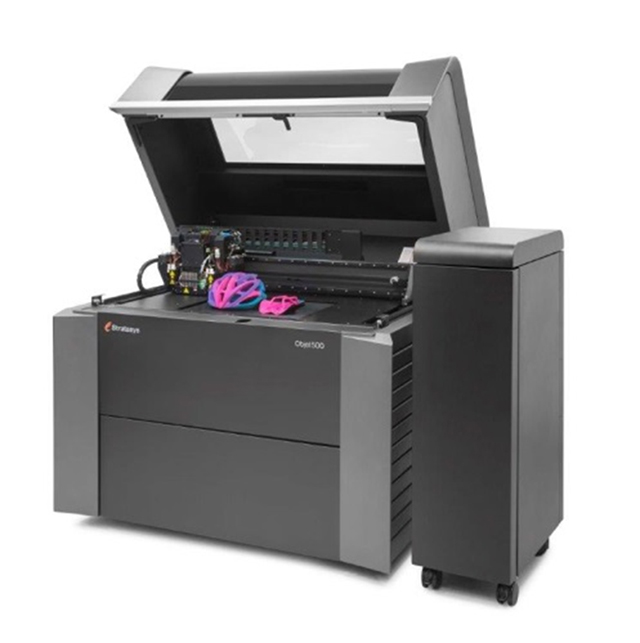
\includegraphics[width=0.90\textwidth]{PrinterI}
			\caption{State of the art $3$D Printers}
			\label{Fig:State of the art $3$D Printers}
		\end{figure}
    \end{column}
    \begin{column}{0.75\textwidth}
    \centering
    \begin{itemize}
			\item Today's $3$D Printers allow for multi-material high resolution prints
			\item Simultaneously multiple objects in varying size can be printed
			\item Voxel-level material assignment enables to reproduce an object's color, shape, texture, gloss,and translucency
			\item Larger print objects are composed of large number of voxels( can easily cross \begin{math}10^{12}\end{math} per object)
		\end{itemize} 
    \end{column}
  \end{columns}
\end{frame}

\subsection{Problem Statement}

\begin{frame}[t]{Why do we need a distributed $3$D Print Driver?}
\begin{columns}
    \begin{column}{0.50\textwidth}
    \centering
    \begin{figure}
			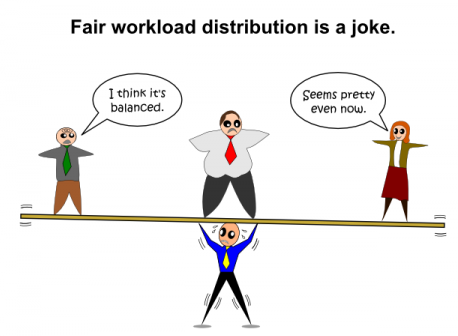
\includegraphics[width=0.90\textwidth]{SillyImage}
			\caption{Distribution Myth}
			\label{Fig:MythI}
		\end{figure}
    \end{column}
    \begin{column}{0.50\textwidth}
    \centering
    \begin{itemize}
    \item Bigger prints require large amount of computational effort 
    \item To fully utilize computational capacity of the work-stations, distribution of the workload is needed  
    \item To allow the distribution of the workload, a distributed printer-driver is required  
		\end{itemize} 
    \end{column}
  \end{columns}
\end{frame}

\section{Solution}

\subsection{Where is the distribution of the workload done?}
\begin{frame}
\begin{columns}
  \begin{column}{0.50\textwidth}
  \centering
    \begin{figure}
			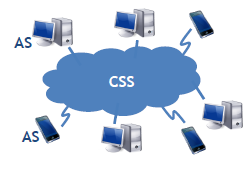
\includegraphics[width=0.90\textwidth]{DistributeIII}
			\caption{Distributed Systems [AS=Autonomous Systems, CSS=Communication Subsystem]}
			\label{Fig:DistributeIII}
		\end{figure}
	\end{column}
	\begin{column}{0.50\textwidth}
  \begin{itemize}
		\item The distribution of the workload is done amongst the nodes of the cluster.
		\item A cluster is a \textbf{\textit{distributed system}} if the workstations are connected to each other by a network and primarily communicate via message passing.(see Fig: \ref{DistributeIII})
	\end{itemize} 
	\end{column}
\end{columns}
\end{frame}

\begin{frame}{Currently used Distributed System}
\begin{columns}
  \begin{column}{0.50\textwidth}
  \centering
    \begin{figure}
			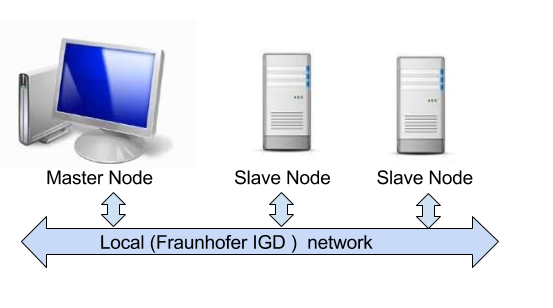
\includegraphics[width=0.90\textwidth]{ArchitectureI}
			\caption{Distributed Systems Architecture}
			\label{Fig:ArchitectureI}
		\end{figure}
	\end{column}
	\begin{column}{0.50\textwidth}
	\begin{itemize}
	\item The distributed system used to implement the solution consists of $3$ nodes - a master nodes and two slave nodes (See Fig: \ref{ArchitectureI})
	\item The nodes are connected via the Fraunhofer network
	\item All the nodes also have access to a shared network file system
	\end{itemize}	
	\end{column}
\end{columns}
\end{frame}

\begin{frame}
\end{frame}

\begin{frame}
\end{frame}

\subsection{How is the distribution done?}
\begin{frame}{Different possibilities of distribution}
\begin{columns}
   \begin{column}{0.50\textwidth}
    \centering
    \begin{figure}
			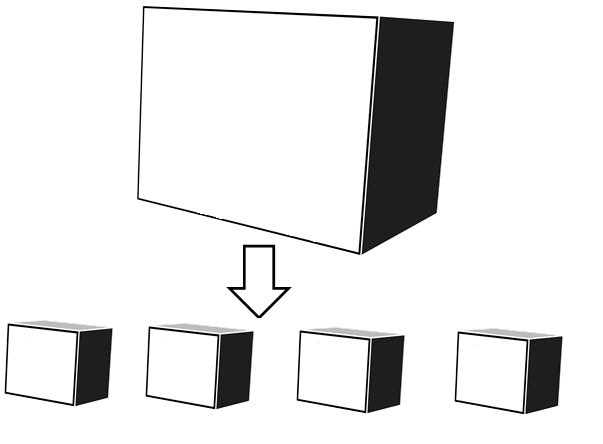
\includegraphics[width=0.30\textwidth]{DistributeI}
			\caption{Distribute Single Large Print Object}
			\label{Fig:DistributeI}
		\end{figure}
		\begin{figure}
			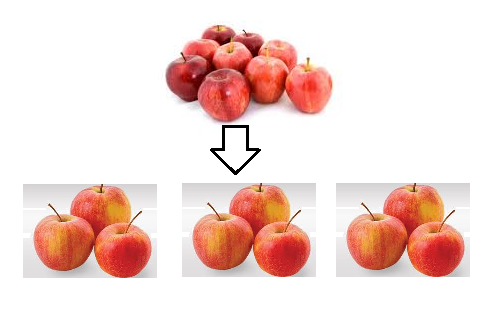
\includegraphics[width=0.70\textwidth]{DistributeII}
			\caption{Distribute Multiple Print Object}
			\label{Fig:DistributeII}
		\end{figure}
   \end{column}
  
	\begin{column}{0.50\textwidth}
    \centering
    \begin{itemize}
		\item Distribute one large print object computation amongst the workstations (see Figure:\ref{Fig:DistributeI})
		\item Distribute multiple print object computation amongst the workstations (see Figure:\ref{Fig:DistributeII})
		\end{itemize} 
    \end{column}
  \end{columns}
  \end{frame}

\begin{frame}{Chosen distribution}
Multiple print objects will be distributed amongst the workstations i.e. each workstation performs computation on one or more inputs
\end{frame}

\begin{frame}{Who distributes the workload?}
\begin{itemize}
\item Streaming architecture
\item Design decisions for distribution 
\end{itemize} 
\end{frame}

\subsection{Gentle Reminder of the Goals}
\section{Current Challenges}
\section{Pending Work}
\section*{Summary}

\begin{frame}
  \frametitle<presentation>{Summary}
\end{frame}

\appendix
\section*{Appendix} 
\end{document}


